\section{Klassifizierung der Graphen} \label{sec:classification}

Nach der Korrelation der Graphen folgt deren Klassifizierung.
Es wird dazu ein Modell entwickelt, welches die Graphen in verschiedene Kategorien klassifiziert.
Die Theorie zur Klassifizierung der Graphen wurde in Kapitel \ref{sec:classification_theory} erläutert. Nun folgen die Anwendung der hergeleiteten Theorie und deren Resultate.

\subsection{Beschreibung des Modells}

Das Modell lehnt sich an das Graph-Convolutional-network (GCN)-Modell von \cite{kipf_semi-supervised_2017} an.
Es besteht aus drei \mintinline{python3}{GCNConv}-Schichten, einer \mintinline{python3}{Pooling}- und einer \mintinline{python3}{Linear}-Schicht.

\begin{figure}[H]
    \centering
    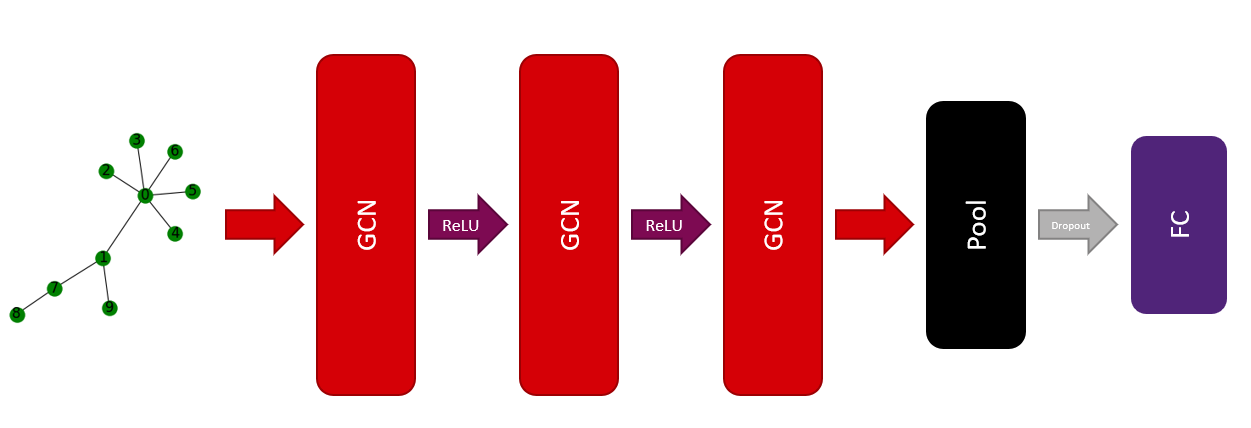
\includegraphics[width=0.8\textwidth]{images/30_results/nn_architecture.png}
    \caption{Modell für die Graphenklassifizierung (Quelle: Eigene Darstellung)}
    \label{fig:model}
\end{figure}

Die Drei \mintinline{python3}{GCNConv}-Schichten sind als Node-Embedding-Schichten zu verstehen.
\begin{equation}
    X' = \hat{D}^{-1/2} \hat{A} \hat{D}^{-1/2} X \Theta
\end{equation}
$\hat{A} = A + I$ ist die Adjazenzmatrix des Graphen mit eingefügten Schleifen $ \hat{D}_{ii} = \sum_{j=0}{\hat{A}_{ij}} $ und der diagonalen Gradmatrix.
Danach folgt eine $ReadOut$-Schicht. Diese existiert, um die einzelnen Node-Embeddings in ein Graph-Embedding zu überführen.
\begin{equation}
    X_{\mathcal{G}} = \frac{1}{\mathcal{V}} \sum_{v \in {\mathcal{V}}}{x_v^{(L)}}
\end{equation}
Es wird mit einer $Dropout$-Schicht \cite{srivastava_dropout_2014} gearbeitet, um Overfitting zu verhindern.
Zum Schluss folgt der Classifier, welcher die Graphen in die Kategorien klassifiziert.

Als Aktivierungsfunktion wird $ ReLU(x) = \max(x, 0) $ verwendet. Die Optimierung der Lernrate erfolgt adaptiv mit $Adam$ \cite{kingma_adam_2017} und dem Parameter $ 0.01 $.
Für die Multi-Class-Klassifizierung wird die Loss-Funktion Crossentropy verwendet.

\subsection{Training des Modells}

Zur Reproduktion und Evaluation folgt die Deklaration der genutzten Hardware und der Daten, die beim Training verwendet wurden.

\begin{table}[H]
    \begin{adjustbox}{minipage=\textwidth, center}
        \scriptsize
        \begin{tabularx}{\textwidth}{|l|X|}
            \hline
            \textbf{Komponente} & \textbf{Beschreibung}                  \\
            \hline
            Prozessor           & AMD Ryzen 9 3900X (24 Cores)           \\
            Arbeitsspeicher     & 64 GB DDR4 3600 MHz                    \\
            Grafikkarte         & NVIDIA GeForce RTX 2080 Ti (CUDA 11.6) \\
            Betriebssystem      & Windows 11 Pro                         \\
            \hline
        \end{tabularx}
    \end{adjustbox}
    \caption{\label{tab:tech-spec}Technische Komponenten für das Training}
\end{table}

Das Datenset besteht aus 3200 Graphen mit verschiedener Anzahl Knoten, siehe Tabelle \ref{data-table}. 
Die Knoten haben jeweils drei Features (Degree, Density und Betweenness), welche für das Node-Embedding verwendet werden.
Die Multi-Class-Klassifizierung hat sieben Klassen (siehe Tabelle \ref{data-table}). Die Graphen werden in 80 \% Trainings- und 20 \% Testdaten aufgeteilt, was eine Trainingsmenge von 2560 Graphen und eine Testmenge von 640 Graphen ergibt.
Die Test- und Trainingsdaten werden in Batches à 64 Graphen unterteilt.

Nach 62 Minuten und 32 Sekunden Training in 170 Epochen, hat das Modell eine Genauigkeit von 93 \% erreicht. 

\begin{listing}[H]
    \begin{minted}[frame=lines,framesep=2mm,baselinestretch=1.2,bgcolor=LightGray,fontsize=\footnotesize,linenos]{text}
        Output exceeds the size limit. Open the full output data in a text editor
        Epoch: 001, Train Acc: 0.1667, Test Acc: 0.1778
        Epoch: 002, Train Acc: 0.2417, Test Acc: 0.2259
        Epoch: 003, Train Acc: 0.3933, Test Acc: 0.3907
        Epoch: 004, Train Acc: 0.5200, Test Acc: 0.5204
        ...
        Epoch: 167, Train Acc: 0.9816, Test Acc: 0.9750
        Epoch: 168, Train Acc: 0.8828, Test Acc: 0.8906
        Epoch: 169, Train Acc: 0.9238, Test Acc: 0.9313
        Epoch: 170, Train Acc: 0.9258, Test Acc: 0.9344
    \end{minted}
    \caption{Verbesserung der Genauigkeit des Modells während des Trainings}
\end{listing}

Im nächsten Bild ist die Genauigkeit über die 170 Epochen dargestellt.
Es ist ersichtlich, dass die Genauigkeit vorwiegend in den ersten 25 Epochen stark zunimmt.
Ab der 100. Epoche gibt es nochmals einen kleinen Anstieg von 0.5 \%.

Auf Abbildung \ref{fig:wandb_dashboard} im Anhang \ref{sec:wandb_dashboard} eine Dashboard-Ansicht von Weights and Biases \cite{wandb}, welches die Genauigkeit und die Loss-Funktion über die Epochen darstellt.
Durch das Hochladen der Trainings- und Testdaten können auch die falschen Klassifizierungen analysiert werden.

\begin{figure}[H]
    \centering
    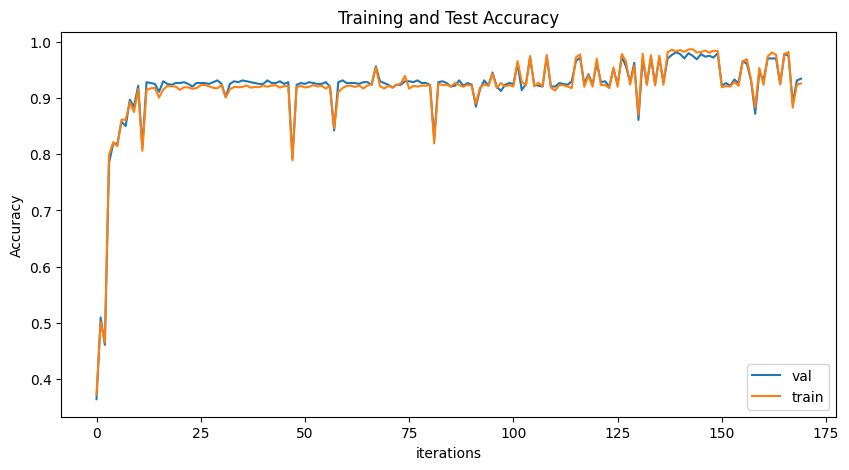
\includegraphics[width=0.8\textwidth]{images/30_results/train_test_acc.png}
    \caption{Genauigkeit des Modells während des Trainings}
    \label{fig:accuracy}
\end{figure}

